\clearpage
\section{典型例题与方案分析}
\label{sec:ch4-worked-examples}

\noindent 本节把原理转化为可检查的计算与判断。计算题先明确符号、激励和读出条件；方案题应完整写出“\textbf{被测量 $\to$ 敏感变化 $\to$ 可测信号}”，并给出使方案成立的材料和环境条件。

\subsection{例题1：应变片的电阻、电流变化与可读性}
\keypoint{复习重点：精确计算相对电流变化，再用绝对变化量与仪表分辨力比较。}

\qs{恒压串联电路中的微小应变}{某应变片初始电阻 $R_0=120\,\Omega$，灵敏度系数 $S_g=2$，受到沿敏感栅方向的\textbf{拉伸应变} $1000\,\mu\varepsilon$。将其与理想毫安表串联后接在 $1.5\,\mathrm V$ 理想直流电源上，求电阻变化、无应变和有应变时的电流、电流表示值的相对变化，并分析能否读出这一变化。}

\sol
\textbf{第一步，把微应变换成无量纲应变。}
\[
\varepsilon=1000\times10^{-6}=10^{-3},\qquad
\frac{\Delta R}{R_0}=S_g\varepsilon=2\times10^{-3}.
\]
因此
\[
\boxed{\Delta R=120\times2\times10^{-3}=0.24\,\Omega},\qquad
R_1=120.24\,\Omega.
\]
受拉时应变为正，按给定 $S_g>0$，电阻增大。

\textbf{第二步，按同一电源电压计算两次电流。}
理想电流表内阻为零，电源内阻及导线电阻忽略，故
\[
\boxed{I_0=\frac{1.5}{120}\,\mathrm A=12.5\,\mathrm{mA}},
\]
\[
\boxed{I_1=\frac{1.5}{120.24}\,\mathrm A
\approx12.47505\,\mathrm{mA}}.
\]
电流减少量为
\[
\Delta I=I_1-I_0\approx-0.0249501\,\mathrm{mA}
=\boxed{-24.9501\,\mu\mathrm A}.
\]

\textbf{第三步，以无应变时的示值为分母。}
\begin{align*}
\frac{\Delta I}{I_0}
&=\frac{U_e/(R_0+\Delta R)-U_e/R_0}{U_e/R_0}\\
&=\frac{R_0}{R_0+\Delta R}-1
=-\frac{\Delta R}{R_0+\Delta R}\\
&=-\frac{S_g\varepsilon}{1+S_g\varepsilon}
=\boxed{-0.001996008\approx-0.199601\%}.
\end{align*}
小量近似为 $\Delta I/I_0\approx-S_g\varepsilon=-0.2\%$，与精确值很接近，但两者不完全相等。

\textbf{第四步，用 $24.95\,\mu\mathrm A$ 判断可读性。}
“毫安表”只说明量级，并未给出量程、最小分度或数字分辨力，因而\textbf{不能仅凭题给信息断言一定能或一定不能读出}。例如：
\begin{itemize}
\item 若 $20\,\mathrm{mA}$ 量程上最小可分辨变化为 $0.1\,\mathrm{mA}$，则本题变化不足一个可分辨单位。
\item 若数字表在合适量程上能分辨 $0.001\,\mathrm{mA}=1\,\mu\mathrm A$，且短期噪声和漂移充分小，则约 $25\,\mu\mathrm A$ 的变化有机会被分辨。
\end{itemize}
分辨出变化还不等于准确测出变化。电源稳定性、接触和导线电阻、表计误差及应变片温漂都会影响结果。实际电源与表计非理想时，可用
\[
I=\frac{U_e}{R_0+\Delta R+R_a+R_s+R_w}
\]
重新建模，$R_a,R_s,R_w$ 分别表示电流表、电源及导线等串联电阻。

\textbf{为什么常用电桥？}直接测电流需从 $12.5\,\mathrm{mA}$ 的背景上分辨约 $0.025\,\mathrm{mA}$ 的变化；平衡电桥可把基准状态调到接近零，再差分放大变化信号。本题若用 $1.5\,\mathrm V$ 激励的单臂等臂桥，则小变化输出大小约为
\[
|U_o|\approx\frac{1.5}{4}\times0.002
=0.00075\,\mathrm V=0.75\,\mathrm{mV}.
\]
这并不自动消除噪声，但给出了便于放大的差分读出形式。

\nt{\textbf{易错：}题设采用拉伸正应变；若改为压缩且 $\varepsilon=-1000\,\mu\varepsilon$，电阻和电流变化方向都会改变。$-0.001996$ 是无量纲相对变化，写成百分数为 $-0.1996\%$。上述理想电流表假设用于电路计算，不能替代实际表计分辨力的规格。}

\Needspace{8cm}
\subsection{例题2：比较电阻、电容与电感的测量电路}
\keypoint{复习重点：共同任务是把参数变化变为可读信号；激励、阻抗性质与主要误差不同。}

\qs{三类参数变化型传感器的共同点与差异}{电阻应变式、电容式、电感式传感器的测量电路有何异同？分别给出一种典型转换方式，并说明读出时需要注意的问题。}

\sol
三者通常都属于\textbf{需要外部激励的参数变化型测量}，被测量先使 $R,C,L$ 改变，再经测量电路变为电压、电流、时间或频率。它们都可采用差动或桥式思想抑制部分共同干扰，并都需要放大、标定及与后级接口匹配。

在交流激励角频率 $\omega_e$ 下，理想元件阻抗分别为
\[
Z_R=R,\qquad Z_L=\iu\omega_eL,\qquad
Z_C=\frac{1}{\iu\omega_eC}.
\]
电阻不依靠储能即可在直流稳态下形成比例电压；电感、电容的交流阻抗与频率有关，因此电路激励条件也是转换关系的一部分。

\begin{table}[H]
\centering\small
\begin{tabularx}{\linewidth}{@{}p{1.7cm} X X@{}}
\toprule
类型 & 典型转换与输出 & 主要误差及处理 \\
\midrule
应变电阻 & 直流或交流电桥：单臂小变化 $|U_o|\approx U_e|\Delta R|/(4R)$。 & 温漂、导线电阻、自热与电源波动；用合理桥臂布置、补偿和稳定激励。 \\
电容 & 交流电桥、充放电计时，或固定 $L$ 的调频电路：$\Delta f/f\approx-\Delta C/(2C)$。 & 电缆和杂散电容、漏电与介质变化；用屏蔽、保护及前置读出。 \\
电感 & 交流电桥、阻抗分压、差动变压器，或固定 $C$ 的调频电路：$\Delta f/f\approx-\Delta L/(2L)$。 & 绕组电阻、磁滞、磁芯温漂、外磁场与损耗；控制激励频率、磁通与环境。 \\
\bottomrule
\end{tabularx}
\end{table}

\textbf{相同的“电桥”并不意味着完全相同的电路。}直流电阻桥比较电阻比例；交流电桥需满足复阻抗平衡，除幅值外还可能涉及相位。交流输出若承载被测量的正负信息，需要相敏检波或其他保留相位的读出方式。

\nt{“电容、电感式只能测动态量”是错误的。静态位移可使 $C$ 或 $L$ 保持在新的值，再由持续交流激励读出。应区分\textbf{被测量的频率}与\textbf{载波激励频率}；同时，电感元件接恒定直流后的稳态电压不能单独用来直接读出 $L$。}

\Needspace{7cm}
\subsection{例题3：光电类型、特点与可测物理量}

\qs{从物理效应到测量方案}{光电传感器有哪些主要类型，各有什么特点？用光电式传感器可以测量哪些物理量？}

\sol
\textbf{先按物理效应分，而不是先按“计数器、测速仪”分。}
\begin{enumerate}
\item \textbf{外光电效应型：}光照使电子逸出表面，典型元件是光电管、光电倍增管。倍增管通过二次发射放大光电流，可检测弱光，但通常需高压供电。
\item \textbf{内光电效应中的光导型：}光照改变内部载流子数量和电导率，如光敏电阻；通常受光后阻值减小，需外电源读出，其线性和响应速度需按元件确认。
\item \textbf{内光电效应中的光生伏特型：}光生载流子在内建电场作用下分离，产生光电流或光电压，如光电池与光伏模式光电二极管；无需外加偏压也能形成光信号输出。
\end{enumerate}

可测量的量不限于光本身，关键在于建立被测量与光之间的关系：
\begin{table}[H]
\centering\small
\begin{tabularx}{\linewidth}{@{}p{3cm} X@{}}
\toprule
被测量 & 转换链示例 \\
\midrule
光强、辐射功率 & 入射光 $\to$ 光电流或电压。 \\
温度 & 目标热辐射 $\to$ 光谱或光强 $\to$ 光电输出，经辐射模型求温度。 \\
位移、尺寸、振动 & 遮光、反射耦合或光斑位置改变 $\to$ 连续输出。 \\
转速、位移增量、数量 & 周期遮光或编码 $\to$ 脉冲频率、相位和计数。 \\
浓度、透明度、浑浊度 & 介质改变吸收、散射或透射 $\to$ 光强或光谱变化。 \\
表面状态、缺陷 & 反射、散射或成像分布改变 $\to$ 强度或图像特征。 \\
\bottomrule
\end{tabularx}
\end{table}

\textbf{选择元件时：}先确定光谱范围与最弱信号，再检查响应速度、噪声、动态范围、线性及背景光。用于通断计数时，稳定跨越阈值比模拟输出严格线性更直接；用于连续光强测量时则必须考虑标定与线性。

\Needspace{8cm}
\subsection{例题4：霍尔效应的解释与三种应用}

\qs{为什么霍尔元件能测多种量}{说明霍尔效应的物理本质，给出三个应用，并区分霍尔元件的直接敏感量与最终被测量。}

\sol
\textbf{物理本质：}通电薄片中的运动载流子受到 $q\mathbf v_d\times\mathbf B$ 的洛伦兹力，向横向偏转；积累电荷建立霍尔电场，直到横向电场力与磁力平衡。于是产生同时垂直于电流与磁场的横向电压，近似满足
\[
U_H=K_HI_bB_\perp.
\]
其中 $I_b$ 是偏置电流；保持它稳定，霍尔电压就反映磁场法向分量。

\begin{enumerate}
\item \textbf{测磁场：}$B_\perp\to U_H$。给定 $K_H=100\,\mathrm{V/(A\,T)}$、$I_b=5\,\mathrm{mA}$，零偏已扣除，若 $U_H=10\,\mathrm{mV}$，则
\[
B_\perp=\frac{0.010}{100\times0.005}=0.020\,\mathrm T.
\]
\item \textbf{测电流：}$I_m\to B_\perp\to U_H$。若磁路已标定为 $B_\perp=k_I I_m$，则 $I_m=U_H/(K_HI_bk_I)$。导线中的被测电流 $I_m$ 与芯片的偏置电流 $I_b$ 不可混同。
\item \textbf{测转速：}$\text{旋转磁体}\to B(t)\to\text{脉冲}\to f_p$。若每周输出两个完整脉冲，测得 $f_p=100\,\mathrm{Hz}$，则 $n=60f_p/2=3000\,\mathrm{r/min}$。该结论以每周脉冲数明确、无漏计为条件。
\end{enumerate}
上述三个例子中，霍尔片直接敏感的都是磁场；电流、转速是通过被测对象与磁场之间的关系间接得到的。测位移时也需引入磁体或磁路，标定 $B(x)$，不能直接把 $U_H\propto B$ 改写为任意范围 $U_H\propto x$。

\nt{霍尔元件可以在恒定磁场下输出电压，磁电感应线圈在磁通不变时输出为零。两者都涉及磁场，但依据的物理机制与适用条件不同。}

\Needspace{8cm}
\subsection{例题5：涡轮机叶片裂纹的多方案检测}
\keypoint{复习重点：方法必须对材料、缺陷位置与探头可达性成立，再说明信号如何形成。}

\qs{为一批叶片设计裂纹检测方案}{有一批涡轮机叶片需要检测裂纹，提出至少两种可行方法，说明传感器原理、可检测的缺陷特点和使用条件。}

\sol
先确认叶片是导电金属、陶瓷还是复合材料，是否有涂层，以及关注表面、近表面还是内部裂纹。以下方法可按对象组合使用。

\subsubsection{方案一：涡流检测导电叶片的表面和近表面裂纹}
交流线圈在导电叶片内激发涡流。裂纹改变涡流路径，使反作用磁场、损耗及探头阻抗变化；检测线圈阻抗的幅值和相位，经扫描定位异常。
\[
\text{裂纹}\to\text{涡流路径改变}\to\Delta Z_{\mathrm{coil}}
\to\text{幅值/相位异常}.
\]
\textbf{适用条件：}叶片材料具有足够导电性，探头能接近表面，缺陷位于有效探测深度内。导电而非铁磁的金属也可使用；常规方法不能直接套用于绝缘陶瓷。应控制或校准曲率、表面涂层、抬离和材质差异，并选择适合缺陷方向的扫描方式与激励频率。

\subsubsection{方案二：压电超声检测内部或一定深度的缺陷}
压电探头施加电压后利用\textbf{逆压电效应}发射超声；超声遇到裂纹等声阻抗突变界面反射，返回波再通过\textbf{正压电效应}转为电信号。脉冲反射法根据异常回波的时间与幅度判断缺陷；若波在材料中往返传播、路径近似直线，深度可由
\[
h=\frac{c_s\Delta t}{2}
\]
估计，$c_s$ 是\textbf{材料中所用声波模式}的传播速度，不能代入空气声速。

\textbf{适用条件：}需有足够声学耦合，探头频率、声束方向和入射角适合叶片形状与缺陷方向。薄壁、强曲率、粗晶材料、近表面盲区和复杂几何可能干扰判读，需多角度、阵列或参考试块辅助。只有声束与裂纹取向合适，才容易获得可识别回波。

\begin{center}
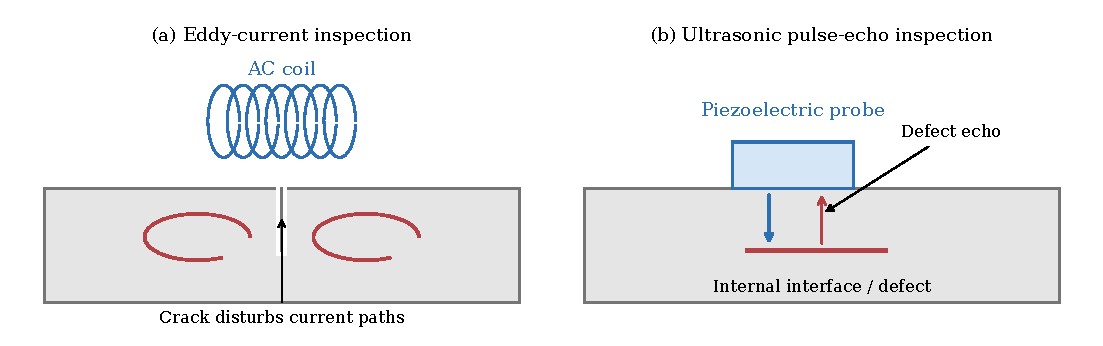
\includegraphics[width=.98\linewidth]{ch4-crack-detection.pdf}
\end{center}
左图中裂纹改变近表层涡流分布；右图中蓝箭头表示发射声波，红箭头表示缺陷回波。示意图只表达机制，实际探头与声束应根据叶片几何布置。

\subsubsection{补充方案：表面光学检测与渗透检测}
光学成像用合适照明和分辨力识别可见表面裂纹。对表面开口、肉眼难辨的裂纹，可用渗透剂进入开口缺陷，再经显像或荧光成像增强对比，光电探测器把光强分布变为图像。其优点是适用于多种致密非多孔材料；限制是只检测\textbf{表面开口}缺陷，需清洁表面并处理涂层遮挡。

若叶片为铁磁性材料，还可考虑磁粉或漏磁检测：磁化后，裂纹扰乱磁通并形成漏磁场，可用磁粉显示或磁敏元件检测。但这类方法\textbf{不能泛用于所有金属或所有叶片}，需先确认铁磁性与可磁化条件。

\begin{table}[H]
\centering\small
\begin{tabularx}{\linewidth}{@{}p{2cm} X X@{}}
\toprule
方法 & 优先关注 & 首先排查的条件 \\
\midrule
涡流 & 导电材料表面、近表面裂纹。 & 导电性、趋肤深度、抬离与曲率。 \\
超声 & 材料内部与适合声束探测的缺陷。 & 耦合、声速、声束方向与几何回波。 \\
光学/渗透 & 可见表面或表面开口裂纹。 & 可见性、光学分辨力、涂层与表面清洁。 \\
磁性方法 & 铁磁材料中的合适取向裂纹。 & 材料磁性、磁化方向与剩磁处理。 \\
\bottomrule
\end{tabularx}
\end{table}

\nt{“检测是否有裂纹”与“定量测出裂纹深度”是不同任务。单次异常信号也可能由材料、边缘或几何变化引起；应以合适参考试样、重复扫描及多方法复核建立判据。}

\Needspace{8cm}
\subsection{例题6：光纤测压力与测位移的异同}

\qs{两种光纤测量是否采用不同的光学效应}{说明光纤传感器测量压力与位移的工作原理，指出两者的不同点，并解释为何不能仅按被测量名称认定光学调制方式。}

\sol
取反射强度式结构作为例子。发射光纤引导光照向反射面，接收光纤收集返回光；间距变化改变光斑几何和耦合效率 $\eta(d)$，故 $P_r=P_t\eta(d)$。

\textbf{位移测量：}反射面就是随被测对象运动的目标，位移直接使间距 $d=d_0\pm x$ 改变。先标定输出与间距关系，再选定单调区域，将输出变化换成位移。

\textbf{压力测量：}反射面设置在受压膜片上，压力先产生弹性变形。若 $x_d=k_pp$，且选取使 $d=d_0-x_d$ 的方向，则小变化灵敏度为
\[
\frac{\diff U_o}{\diff p}
=\frac{\diff U_o}{\diff P_r}\,
P_t\frac{\diff\eta}{\diff d}\,
\frac{\diff d}{\diff p}
=-\frac{\diff U_o}{\diff P_r}\,
P_t\frac{\diff\eta}{\diff d}\,k_p.
\]
因此压力灵敏度同时取决于光学读出斜率与膜片的机械灵敏度；输出方向也由选定的光强曲线分支决定。

\begin{table}[H]
\centering\small
\begin{tabularx}{\linewidth}{@{}p{2.2cm} X X@{}}
\toprule
比较项 & 测位移 & 测压力 \\
\midrule
直接机械输入 & 目标自身位移。 & 压力对膜片或弹性体的作用。 \\
机械变换 & 通常直接改变光学间距。 & 先经 $p\to x_d$ 或 $p\to\varepsilon$。 \\
共同光学过程 & \multicolumn{2}{l@{}}{可共用强度、相位或波长调制与光电读出。} \\
额外标定因素 & 反射率、光源、光路和工作区。 & 除左列外，还需膜片刚度、有效面积、温度及压力边界条件。 \\
\bottomrule
\end{tabularx}
\end{table}

压力也可使FBG应变、引起反射波长漂移；位移也可改变干涉腔长度、引起相位变化。两者的根本差别是\textbf{被测量与光学敏感量之间的机械转换关系}，并不存在“压力只能调相位、位移只能调强度”的普遍规定。

\Needspace{8cm}
\subsection{例题7：把选型原则用于一个完整任务}

\qs{为机器人末端选择力传感器}{机器人末端需要监测缓慢变化的夹持力，并在接触瞬间检测冲击；传感器安装空间有限，现场存在电机电磁干扰。应怎样比较候选方案？}

\sol
\textbf{首先明确两个频率范围。}夹持力包含近直流成分，冲击包含较高频成分；同一方案须兼顾静态稳定性与动态带宽，或采用互补方案。

\begin{enumerate}
\item \textbf{先检查可测性：}应变电阻式、合适电容式或FBG弹性体可作为持续夹持力的候选；压电式适合冲击，但单独用于长期恒力会受电荷泄漏限制。
\item \textbf{再定范围与分辨力：}按最大夹持力及冲击过载留量程裕量；由最小有意义的力变化确定所需输入分辨力，并将噪声与温漂折算回力输入。
\item \textbf{核查动态与结构：}查整体弹性体、质量与安装连接的动态响应，使关注频带内的幅相误差满足要求；不要只用敏感材料“响应快”代替整机核查。
\item \textbf{比较环境和接口：}应变桥可用差分放大、屏蔽和合理布线减轻电机干扰；FBG有抗电磁干扰优势，但需光学解调与温度补偿；电容方案需关注寄生电容、污染与布线。
\item \textbf{确定可标定性和维护成本：}按实际安装状态进行零点、量程、重复性、回程和多轴交叉敏感标定，比较体积、成本、寿命与更换便利性。
\end{enumerate}

可形成“应变式弹性体监测持续夹持力，带宽和过载经验证后兼顾冲击”的方案；若冲击频段超出该结构的可用频带，可增加压电通道。若电磁环境和布线使电测方案难以达到误差目标，则进一步比较FBG。\textbf{没有明确量程、频带与误差指标时，原则能给出筛选方向，不能唯一决定型号。}

\nt{选型不是把灵敏度、精度和带宽都取最大值。应检查它们是否满足任务，并明确为了灵敏度、量程、鲁棒性和成本所作的取舍。}
